\documentclass[11pt,preprint]{elsarticle}

\usepackage{lmodern}
%%%% My spacing
\usepackage{setspace}
\setstretch{1.2}
\DeclareMathSizes{12}{14}{10}{10}

% Wrap around which gives all figures included the [H] command, or places it "here". This can be tedious to code in Rmarkdown.
\usepackage{float}
\let\origfigure\figure
\let\endorigfigure\endfigure
\renewenvironment{figure}[1][2] {
    \expandafter\origfigure\expandafter[H]
} {
    \endorigfigure
}

\let\origtable\table
\let\endorigtable\endtable
\renewenvironment{table}[1][2] {
    \expandafter\origtable\expandafter[H]
} {
    \endorigtable
}


\usepackage{ifxetex,ifluatex}
\usepackage{fixltx2e} % provides \textsubscript
\ifnum 0\ifxetex 1\fi\ifluatex 1\fi=0 % if pdftex
  \usepackage[T1]{fontenc}
  \usepackage[utf8]{inputenc}
\else % if luatex or xelatex
  \ifxetex
    \usepackage{mathspec}
    \usepackage{xltxtra,xunicode}
  \else
    \usepackage{fontspec}
  \fi
  \defaultfontfeatures{Mapping=tex-text,Scale=MatchLowercase}
  \newcommand{\euro}{€}
\fi

\usepackage{amssymb, amsmath, amsthm, amsfonts}

\def\bibsection{\section*{References}} %%% Make "References" appear before bibliography


\usepackage[numbers]{natbib}

\usepackage{longtable}
\usepackage[margin=2.3cm,bottom=2cm,top=2.5cm, includefoot]{geometry}
\usepackage{fancyhdr}
\usepackage[bottom, hang, flushmargin]{footmisc}
\usepackage{graphicx}
\numberwithin{equation}{section}
\numberwithin{figure}{section}
\numberwithin{table}{section}
\setlength{\parindent}{0cm}
\setlength{\parskip}{1.3ex plus 0.5ex minus 0.3ex}
\usepackage{textcomp}
\renewcommand{\headrulewidth}{0.2pt}
\renewcommand{\footrulewidth}{0.3pt}

\usepackage{array}
\newcolumntype{x}[1]{>{\centering\arraybackslash\hspace{0pt}}p{#1}}

%%%%  Remove the "preprint submitted to" part. Don't worry about this either, it just looks better without it:
\makeatletter
\def\ps@pprintTitle{%
  \let\@oddhead\@empty
  \let\@evenhead\@empty
  \let\@oddfoot\@empty
  \let\@evenfoot\@oddfoot
}
\makeatother

 \def\tightlist{} % This allows for subbullets!

\usepackage{hyperref}
\hypersetup{breaklinks=true,
            bookmarks=true,
            colorlinks=true,
            citecolor=blue,
            urlcolor=blue,
            linkcolor=blue,
            pdfborder={0 0 0}}


% The following packages allow huxtable to work:
\usepackage{siunitx}
\usepackage{multirow}
\usepackage{hhline}
\usepackage{calc}
\usepackage{tabularx}
\usepackage{booktabs}
\usepackage{caption}


\newenvironment{columns}[1][]{}{}

\newenvironment{column}[1]{\begin{minipage}{#1}\ignorespaces}{%
\end{minipage}
\ifhmode\unskip\fi
\aftergroup\useignorespacesandallpars}

\def\useignorespacesandallpars#1\ignorespaces\fi{%
#1\fi\ignorespacesandallpars}

\makeatletter
\def\ignorespacesandallpars{%
  \@ifnextchar\par
    {\expandafter\ignorespacesandallpars\@gobble}%
    {}%
}
\makeatother


% definitions for citeproc citations
\NewDocumentCommand\citeproctext{}{}
\NewDocumentCommand\citeproc{mm}{%
\href{\#cite.\detokenize{#1}}{#2}\nocite{#1}}

\makeatletter
% allow citations to break across lines
\let\@cite@ofmt\@firstofone
% avoid brackets around text for \cite:
\def\@biblabel#1{}
\def\@cite#1#2{{#1\if@tempswa , #2\fi}}
\makeatother
\newlength{\cslhangindent}
\setlength{\cslhangindent}{1.5em}
\newlength{\csllabelwidth}
\setlength{\csllabelwidth}{3em}
\newenvironment{CSLReferences}[2] % #1 hanging-indent, #2 entry-spacing
{\begin{list}{}{%
	\setlength{\itemindent}{0pt}
	\setlength{\leftmargin}{0pt}
	\setlength{\parsep}{0pt}
	% turn on hanging indent if param 1 is 1
	\ifodd #1
	\setlength{\leftmargin}{\cslhangindent}
	\setlength{\itemindent}{-1\cslhangindent}
	\fi
	% set entry spacing
	\setlength{\itemsep}{#2\baselineskip}}}
{\end{list}}

\usepackage{calc}
\newcommand{\CSLBlock}[1]{\hfill\break\parbox[t]{\linewidth}{\strut\ignorespaces#1\strut}}
\newcommand{\CSLLeftMargin}[1]{\parbox[t]{\csllabelwidth}{\strut#1\strut}}
\newcommand{\CSLRightInline}[1]{\parbox[t]{\linewidth - \csllabelwidth}{\strut#1\strut}}
\newcommand{\CSLIndent}[1]{\hspace{\cslhangindent}#1}


\urlstyle{same}  % don't use monospace font for urls
\setlength{\parindent}{0pt}
\setlength{\parskip}{6pt plus 2pt minus 1pt}
\setlength{\emergencystretch}{3em}  % prevent overfull lines
\setcounter{secnumdepth}{5}

%%% Use protect on footnotes to avoid problems with footnotes in titles
\let\rmarkdownfootnote\footnote%
\def\footnote{\protect\rmarkdownfootnote}
\IfFileExists{upquote.sty}{\usepackage{upquote}}{}

%%% Include extra packages specified by user
\usepackage{array}
\usepackage{caption}
\usepackage{graphicx}
\usepackage{siunitx}
\usepackage[normalem]{ulem}
\usepackage{colortbl}
\usepackage{multirow}
\usepackage{hhline}
\usepackage{calc}
\usepackage{tabularx}
\usepackage{threeparttable}
\usepackage{wrapfig}
\usepackage{adjustbox}
\usepackage{hyperref}

%%% Hard setting column skips for reports - this ensures greater consistency and control over the length settings in the document.
%% page layout
%% paragraphs
\setlength{\baselineskip}{12pt plus 0pt minus 0pt}
\setlength{\parskip}{12pt plus 0pt minus 0pt}
\setlength{\parindent}{0pt plus 0pt minus 0pt}
%% floats
\setlength{\floatsep}{12pt plus 0 pt minus 0pt}
\setlength{\textfloatsep}{20pt plus 0pt minus 0pt}
\setlength{\intextsep}{14pt plus 0pt minus 0pt}
\setlength{\dbltextfloatsep}{20pt plus 0pt minus 0pt}
\setlength{\dblfloatsep}{14pt plus 0pt minus 0pt}
%% maths
\setlength{\abovedisplayskip}{12pt plus 0pt minus 0pt}
\setlength{\belowdisplayskip}{12pt plus 0pt minus 0pt}
%% lists
\setlength{\topsep}{10pt plus 0pt minus 0pt}
\setlength{\partopsep}{3pt plus 0pt minus 0pt}
\setlength{\itemsep}{5pt plus 0pt minus 0pt}
\setlength{\labelsep}{8mm plus 0mm minus 0mm}
\setlength{\parsep}{\the\parskip}
\setlength{\listparindent}{\the\parindent}
%% verbatim
\setlength{\fboxsep}{5pt plus 0pt minus 0pt}



\begin{document}



\begin{frontmatter}  %

\title{Billionaires : Self-made or Daddy-made}

% Set to FALSE if wanting to remove title (for submission)




\author[Add1]{Tagishi Mashego}
\ead{}








\vspace{1cm}





\vspace{0.5cm}

\end{frontmatter}

\setcounter{footnote}{0}



%________________________
% Header and Footers
%%%%%%%%%%%%%%%%%%%%%%%%%%%%%%%%%
\pagestyle{fancy}
\chead{}
\rhead{}
\lfoot{}
\rfoot{\footnotesize Page \thepage}
\lhead{}
%\rfoot{\footnotesize Page \thepage } % "e.g. Page 2"
\cfoot{}

%\setlength\headheight{30pt}
%%%%%%%%%%%%%%%%%%%%%%%%%%%%%%%%%
%________________________

\headsep 35pt % So that header does not go over title




\section{Answer}\label{answer}

\subsection{Part 1}\label{part-1}

\begin{figure}[H]

{\centering 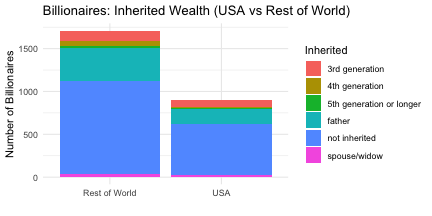
\includegraphics{Question4_files/figure-latex/Figure1-1} 

}

\caption{Billionaire Comparison \label{Figure1}}\label{fig:Figure1}
\end{figure}

Kudos to the Americans , they have really created an economy that
conducive for generating Uber wealth. Unfortunately, the notion held
that those who are rich in America are only hard-nosed workaholics who
built businesses from scratch, while the rest of the world's
billionaires inherit their wealth , is simply not true.

Figure \ref{Figure1} shows that the Rest of the World has more self-made
billionaires than the USA, yes the rest of the world has more
billionaires who have inherited that wealth too, but we see that both
can be true. Surely one might surmise that this hold purely based on the
fact that the Rest of the World has more people than the USA , the next
figure will address that thought.

Table \ref{tab1} shows that over two-thirds of American billionaires
over the history of time are self-made, dispelling any false notions
that there is an entrepreneurial gene. Another noteworthy figure is the
number of those who inherited via 5th generation or longer, as this
family has been through depressions , recessions and yet maintains
billionaire status.

\begin{table}[ht]
\centering
\begin{tabular}{lrr}
  \hline
wealth.how.inherited & count & percentage \\ 
  \hline
not inherited & 597 & 66.10 \\ 
  father & 177 & 19.60 \\ 
  3rd generation &  84 & 9.30 \\ 
  spouse/widow &  24 & 2.70 \\ 
  4th generation &  11 & 1.20 \\ 
  5th generation or longer &  10 & 1.10 \\ 
   \hline
\end{tabular}
\caption{USA Billionaires by Inheritance Status \label{tab1}} 
\end{table}

Looking at Table \ref{tab2} we see that the rest of the world has a
slightly lower percentage of self-made billionaires at 63.8\% . This is
a narrative that the Americans are running with and I hate to be the one
to confirm it.

\begin{table}[ht]
\centering
\begin{tabular}{lrr}
  \hline
wealth.how.inherited & count & percentage \\ 
  \hline
not inherited & 1091 & 63.80 \\ 
  father & 381 & 22.30 \\ 
  3rd generation & 126 & 7.40 \\ 
  4th generation &  57 & 3.30 \\ 
  spouse/widow &  35 & 2.00 \\ 
  5th generation or longer &  21 & 1.20 \\ 
   \hline
\end{tabular}
\caption{Rest of the World by Inheritance Status\label{tab2}} 
\end{table}

\newpage

As quants we aim to steer our clients to invest in companies that are
profitable.Table \ref{tab3} uses the number of billionaires associated
with a company as a proxy for the profitability of the company , with 4
of the top 5 companies being US based it is no wonder the US is a
certified economic powerhouse.

\begin{table}[ht]
\centering
\begin{tabular}{lrl}
  \hline
company.name & total\_billionaires & region \\ 
  \hline
Walmart &  18 & USA \\ 
  Campbell Soup &  16 & USA \\ 
  Hyatt &  15 & USA \\ 
  SAP AG &  12 & Rest of World \\ 
  Microsoft &  11 & USA \\ 
   \hline
\end{tabular}
\caption{Companies With Most Billionaires \label{tab3}} 
\end{table}

\subsection{Part 2}\label{part-2}

The year 2000 is widely regarded as the peak of the dot.com bubble , a
period where technology startups saw immense growth and profits.
Unfortunately , it came to an end known as the bubble `burst' in the
early 2000, but does that mean incredibly successful tech startups are a
thing of the past?

\begin{figure}[H]

{\centering 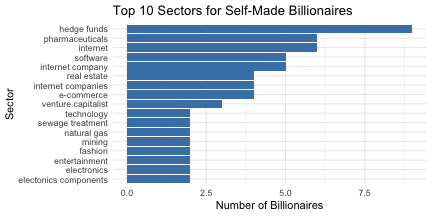
\includegraphics{Question4_files/figure-latex/Figure2-1} 

}

\caption{Companies founded Since 2000 \label{Figure2}}\label{fig:Figure2}
\end{figure}

Figure \ref{Figure2} shows that the technology sector remains
strong---ranking as the fourth most common source of billionaire-founded
companies since 2000. However, it trails behind consumer services type
sectors such as pharmaceuticals.

\hfill

\section*{References}\label{references}
\addcontentsline{toc}{section}{References}

\phantomsection\label{refs}
\begin{CSLReferences}{1}{1}
\bibitem[\citeproctext]{ref-Texevier}
Katzke, N.F. 2017. \emph{{Texevier}: {P}ackage to create elsevier
templates for rmarkdown}. Stellenbosch, South Africa: Bureau for
Economic Research.

\end{CSLReferences}

\section*{Appendix}\label{appendix}
\addcontentsline{toc}{section}{Appendix}

\subsection*{Appendix A}\label{appendix-a}
\addcontentsline{toc}{subsection}{Appendix A}

Some appendix information here

\subsection*{Appendix B}\label{appendix-b}
\addcontentsline{toc}{subsection}{Appendix B}

Katzke (\citeproc{ref-Texevier}{2017})

\bibliography{Tex/ref}





\end{document}
